

\tikzset{every picture/.style={line width=0.75pt}} %set default line width to 0.75pt        

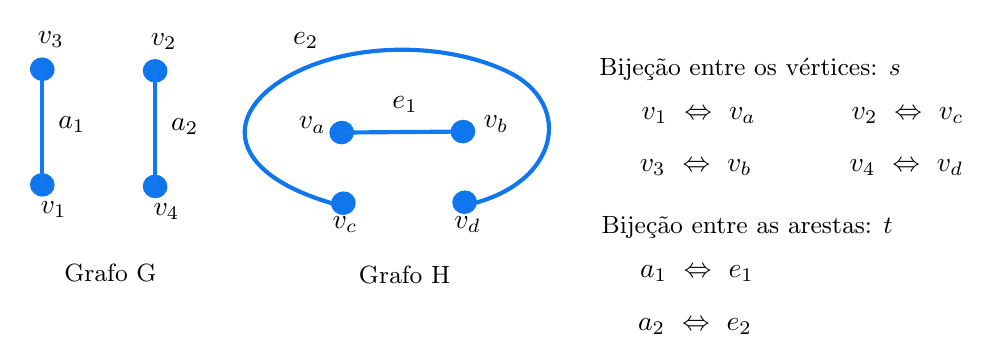
\begin{tikzpicture}[x=0.75pt,y=0.75pt,yscale=-1,xscale=1]
%uncomment if require: \path (0,187); %set diagram left start at 0, and has height of 187

%Curve Lines [id:da13535893571863644] 
\draw [color={rgb, 255:red, 15; green, 118; blue, 237 }  ,draw opacity=1 ][line width=1.5]    (221.9,92.91) .. controls (267.74,83.37) and (275.04,43.91) .. (242.59,28.44) .. controls (210.14,12.96) and (161.46,14.51) .. (133.06,33.08) .. controls (104.67,51.65) and (109.53,79.5) .. (163.49,93.38) ;
%Shape: Ellipse [id:dp4051450804535437] 
\draw  [draw opacity=0][fill={rgb, 255:red, 15; green, 118; blue, 237 }  ,fill opacity=1 ] (14.2,23.2) .. controls (16.51,21.01) and (20.28,21.07) .. (22.62,23.32) .. controls (24.95,25.58) and (24.96,29.17) .. (22.64,31.35) .. controls (20.33,33.54) and (16.56,33.48) .. (14.23,31.23) .. controls (11.89,28.97) and (11.88,25.38) .. (14.2,23.2) -- cycle ;
%Shape: Ellipse [id:dp9979632274073846] 
\draw  [draw opacity=0][fill={rgb, 255:red, 15; green, 118; blue, 237 }  ,fill opacity=1 ] (14.2,78.9) .. controls (16.51,76.72) and (20.28,76.78) .. (22.62,79.03) .. controls (24.95,81.28) and (24.96,84.88) .. (22.64,87.06) .. controls (20.33,89.24) and (16.56,89.19) .. (14.23,86.93) .. controls (11.89,84.68) and (11.88,81.09) .. (14.2,78.9) -- cycle ;
%Straight Lines [id:da7110634067887398] 
\draw [color={rgb, 255:red, 16; green, 121; blue, 243 }  ,draw opacity=1 ][fill={rgb, 255:red, 0; green, 0; blue, 0 }  ,fill opacity=1 ][line width=1.5]    (18.42,27.27) -- (18.42,82.98) ;
%Shape: Ellipse [id:dp37656452184529754] 
\draw  [draw opacity=0][fill={rgb, 255:red, 15; green, 118; blue, 237 }  ,fill opacity=1 ] (68.56,23.97) .. controls (70.87,21.79) and (74.64,21.84) .. (76.98,24.1) .. controls (79.31,26.35) and (79.32,29.94) .. (77,32.13) .. controls (74.69,34.31) and (70.92,34.25) .. (68.58,32) .. controls (66.25,29.75) and (66.24,26.15) .. (68.56,23.97) -- cycle ;
%Shape: Ellipse [id:dp8237350008256439] 
\draw  [draw opacity=0][fill={rgb, 255:red, 15; green, 118; blue, 237 }  ,fill opacity=1 ] (68.56,79.68) .. controls (70.87,77.49) and (74.64,77.55) .. (76.98,79.8) .. controls (79.31,82.06) and (79.32,85.65) .. (77,87.83) .. controls (74.69,90.02) and (70.92,89.96) .. (68.58,87.71) .. controls (66.25,85.45) and (66.24,81.86) .. (68.56,79.68) -- cycle ;
%Straight Lines [id:da9589476920573761] 
\draw [color={rgb, 255:red, 16; green, 121; blue, 243 }  ,draw opacity=1 ][fill={rgb, 255:red, 0; green, 0; blue, 0 }  ,fill opacity=1 ][line width=1.5]    (72.78,28.05) -- (72.78,83.76) ;
%Shape: Ellipse [id:dp7592445989982248] 
\draw  [draw opacity=0][fill={rgb, 255:red, 15; green, 118; blue, 237 }  ,fill opacity=1 ] (158.43,61.85) .. controls (156.13,59.66) and (156.15,56.07) .. (158.49,53.82) .. controls (160.84,51.58) and (164.61,51.54) .. (166.91,53.73) .. controls (169.22,55.92) and (169.19,59.51) .. (166.85,61.76) .. controls (164.51,64) and (160.74,64.04) .. (158.43,61.85) -- cycle ;
%Shape: Ellipse [id:dp46395815979252064] 
\draw  [draw opacity=0][fill={rgb, 255:red, 15; green, 118; blue, 237 }  ,fill opacity=1 ] (216.85,61.38) .. controls (214.54,59.19) and (214.57,55.59) .. (216.91,53.35) .. controls (219.25,51.1) and (223.02,51.06) .. (225.33,53.25) .. controls (227.64,55.44) and (227.61,59.04) .. (225.27,61.28) .. controls (222.92,63.53) and (219.15,63.57) .. (216.85,61.38) -- cycle ;
%Straight Lines [id:da10247453238790105] 
\draw [color={rgb, 255:red, 16; green, 121; blue, 243 }  ,draw opacity=1 ][fill={rgb, 255:red, 0; green, 0; blue, 0 }  ,fill opacity=1 ][line width=1.5]    (162.67,57.79) -- (221.09,57.31) ;
%Shape: Ellipse [id:dp3514904288568135] 
\draw  [draw opacity=0][fill={rgb, 255:red, 15; green, 118; blue, 237 }  ,fill opacity=1 ] (159.24,95.9) .. controls (156.94,93.71) and (156.96,90.11) .. (159.31,87.87) .. controls (161.65,85.62) and (165.42,85.58) .. (167.73,87.77) .. controls (170.03,89.96) and (170.01,93.56) .. (167.66,95.8) .. controls (165.32,98.05) and (161.55,98.09) .. (159.24,95.9) -- cycle ;
%Shape: Ellipse [id:dp7592627436182027] 
\draw  [draw opacity=0][fill={rgb, 255:red, 15; green, 118; blue, 237 }  ,fill opacity=1 ] (217.66,95.42) .. controls (215.35,93.23) and (215.38,89.63) .. (217.72,87.39) .. controls (220.06,85.15) and (223.83,85.1) .. (226.14,87.3) .. controls (228.45,89.49) and (228.42,93.08) .. (226.08,95.33) .. controls (223.73,97.57) and (219.97,97.61) .. (217.66,95.42) -- cycle ;

% Text Node
\draw (14.82,7.76) node [anchor=north west][inner sep=0.75pt]    {$v_{3}$};
% Text Node
\draw (16.15,89.62) node [anchor=north west][inner sep=0.75pt]    {$v_{1}$};
% Text Node
\draw (24.65,48.76) node [anchor=north west][inner sep=0.75pt]    {$a_{1}$};
% Text Node
\draw (69.18,8.53) node [anchor=north west][inner sep=0.75pt]    {$v_{2}$};
% Text Node
\draw (70.51,90.39) node [anchor=north west][inner sep=0.75pt]    {$v_{4}$};
% Text Node
\draw (79.01,49.54) node [anchor=north west][inner sep=0.75pt]    {$a_{2}$};
% Text Node
\draw (27.53,119.56) node [anchor=north west][inner sep=0.75pt]  [font=\small] [align=left] {Grafo G};
% Text Node
\draw (140.6,48.8) node [anchor=north west][inner sep=0.75pt]  [rotate=-0.23]  {$v_{a}$};
% Text Node
\draw (229.62,48.34) node [anchor=north west][inner sep=0.75pt]  [rotate=-0.45]  {$v_{b}$};
% Text Node
\draw (185.57,38.85) node [anchor=north west][inner sep=0.75pt]  [rotate=-359.74]  {$e_{1}$};
% Text Node
\draw (137.7,7.9) node [anchor=north west][inner sep=0.75pt]  [rotate=-359.74]  {$e_{2}$};
% Text Node
\draw (156.83,96.77) node [anchor=north west][inner sep=0.75pt]  [rotate=-0.23]  {$v_{c}$};
% Text Node
\draw (215.52,96.56) node [anchor=north west][inner sep=0.75pt]  [rotate=-0.23]  {$v_{d}$};
% Text Node
\draw (169.51,120.76) node [anchor=north west][inner sep=0.75pt]  [font=\small] [align=left] {Grafo H};
% Text Node
\draw (285.35,20.41) node [anchor=north west][inner sep=0.75pt]  [font=\small] [align=left] {Bijeção entre os vértices: $\displaystyle s$};
% Text Node
\draw (286.41,96.79) node [anchor=north west][inner sep=0.75pt]  [font=\small] [align=left] {Bijeção entre as arestas: $\displaystyle t$};
% Text Node
\draw (305.74,44.17) node [anchor=north west][inner sep=0.75pt]    {$v_{1} \ \Leftrightarrow \ v_{a}$};
% Text Node
\draw (304.8,69.33) node [anchor=north west][inner sep=0.75pt]    {$v_{3} \ \Leftrightarrow \ v_{b}$};
% Text Node
\draw (406.88,44.17) node [anchor=north west][inner sep=0.75pt]    {$v_{2} \ \Leftrightarrow \ v_{c}$};
% Text Node
\draw (405.91,69.33) node [anchor=north west][inner sep=0.75pt]    {$v_{4} \ \Leftrightarrow \ v_{d}$};
% Text Node
\draw (304.9,120.55) node [anchor=north west][inner sep=0.75pt]    {$a_{1} \ \Leftrightarrow \ e_{1}$};
% Text Node
\draw (303.96,145.71) node [anchor=north west][inner sep=0.75pt]    {$a_{2} \ \Leftrightarrow \ e_{2}$};


\end{tikzpicture}
